\documentclass[10pt]{beamer}
\usetheme{Marburg}
\graphicspath{{Arquivos/}}
\usepackage[utf8]{inputenc}
\usepackage[french]{babel}
\usepackage[T1]{fontenc}
\usepackage{amsmath}
\usepackage{amsfonts}
\usepackage{amssymb}
\usepackage{graphicx}
\usepackage{hyperref}
\author{Anita Klein - Mariam Grigoryan - Steve de Rose}
\title{Airborne Transmission of Covid-19}
\date{}

\begin{document}
    
\begin{frame}
    \maketitle
\end{frame}

\begin{frame}{The Concept}
    \begin{itemize}
        \item Covid 19 virus reported to the World Health Organization (WHO) on December 31, 2019. 
        \item Reduce/Prevent its spread
        \item Cemosis and Synapse-Concept project 4fastsim-ibat. 
        \item Air quality since Covid-19.
    \end{itemize}
\end{frame}

\begin{frame}{Collaboration Cemosis/Synapse}
    \begin{itemize}
        \item Cemosis created in January 2013 by Christophe Prud’homme. 
        \item Strasbourg Centre for Modelling and Simulation.
        \item Synapse-Concept created in November 1999.
        \item Specialised in engineering and technical studies.
    \end{itemize}
\end{frame}

\begin{frame}{Project}
    \begin{itemize}
        \item Study of the airborne transmission of COVID-19 in an indoor space.
        \item The air in the room follows an advection-diffusion-reaction equation.
        \item With only one infectious person in the room.
        \item Rome of size $8m(l)\times 8m(w) \times 3m(h)$.
        \item Breathing/Talking with and without a face mask.
    \end{itemize}
\end{frame}

\begin{frame}{Illustration}
        \begin{figure}
            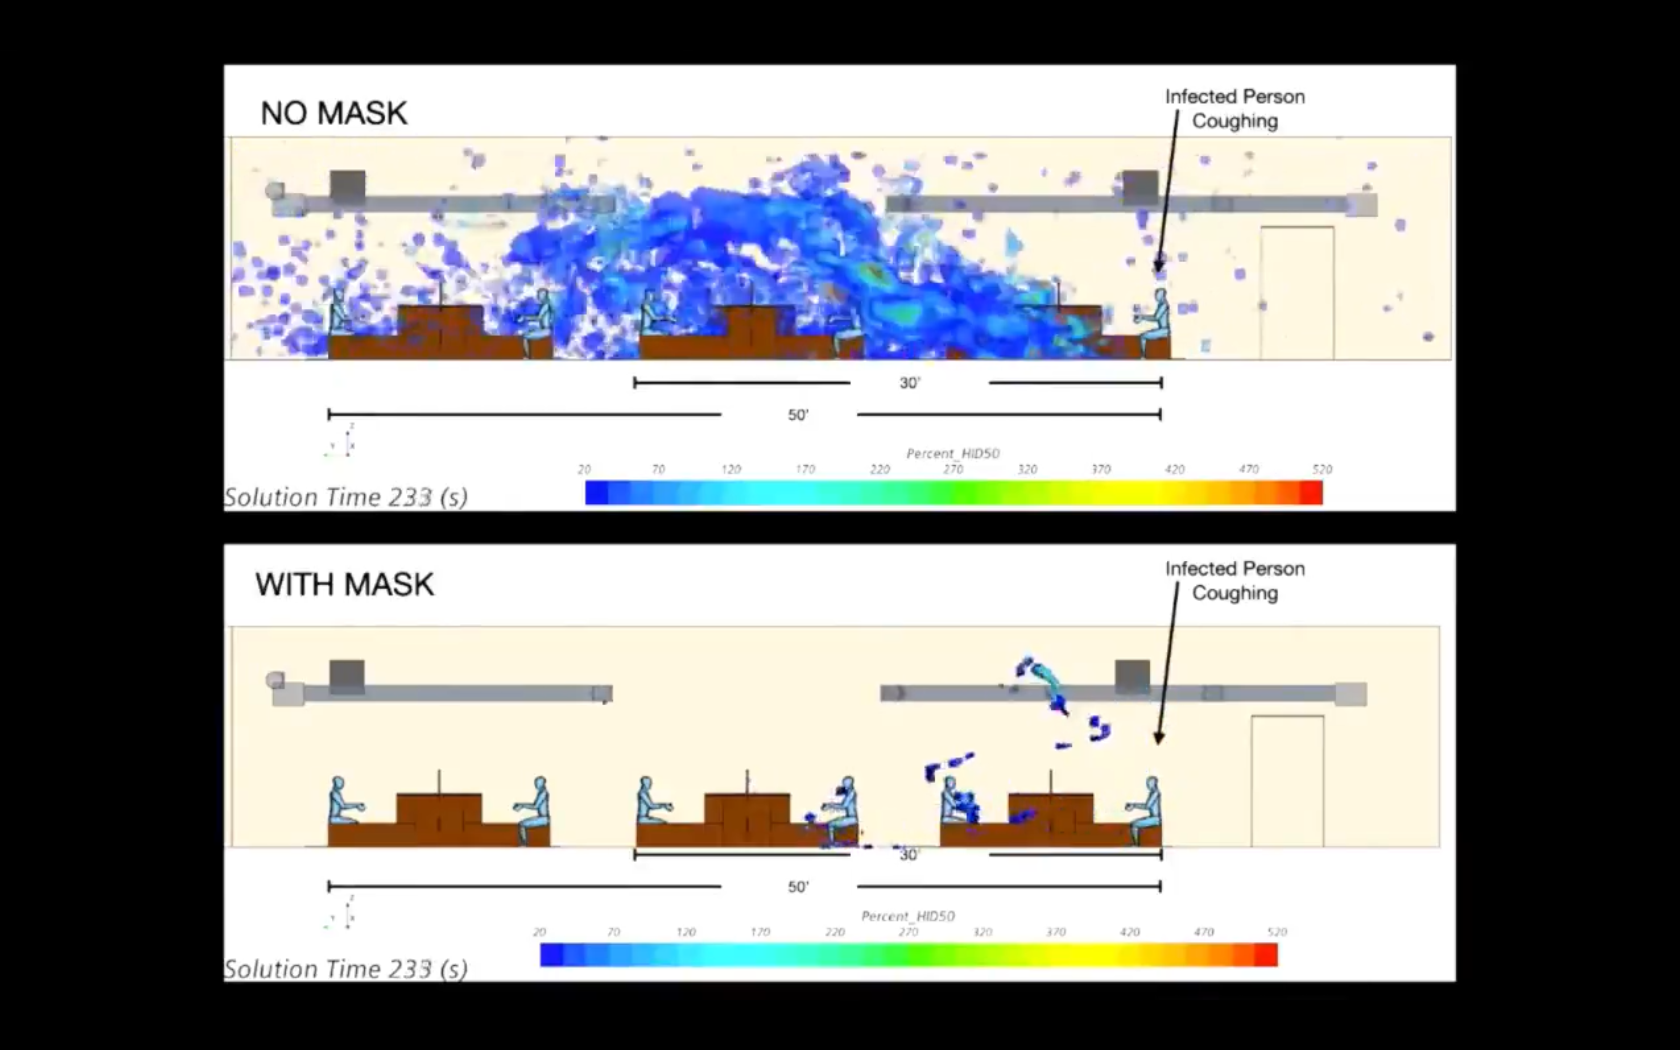
\includegraphics[width=\textwidth]{illu.png}
            \caption{Virus airborne transmission in an office }
        \end{figure}  
\end{frame}

\begin{frame}{Methodology I}
    \begin{itemize}
        \item Firstly, 2D model to study/reproduce the concentration of airborne infectious particles.
        \item Using the advection–reaction–diffusion equation.
        \item Assumptions: \\- particles  released from
        the infected person with zero initial velocity.
        \\ - transported via advection due to the airflow in the room and diffusion due to turbulent mixing
        \\ - the advection velocity of the air, $v (m/s)$ controlled by the air-conditioning unit.
        \\ -  the recirculation of air leads to turbulent mixing of the infectious particles.  
    \end{itemize}  

\end{frame}

\begin{frame}{ARD Equation}
    \begin{itemize}
        \item Hence, the advection–reaction–diffusion equation :
        \\ $$ \frac{\partial C}{\partial t} = \nabla . (K  \nabla  C) - \nabla . (\overrightarrow{v}  C) + S.$$
        \item C = concentration of airborne infectious particles \\
        t = time \\
        $\nabla$ = two-dimensional gradient operator \\
        K = isotropic eddy diffusion coefficient (turbulent diffusion ) \\
        $\overrightarrow{v}$ = advection velocity of the air \\
        S = sum of sources and sinks of viral particles.
    \end{itemize}  

\end{frame}

\begin{frame}{Methodology II}
    \begin{itemize}
        \item Secondly, using «N-point ASOM» (air supply opening model).
        \item Developped in 2003 by Bin Zhaoa, Xianting Lib and Qisen Yanb at Tsinghua University, Beijing, China. 
        \item Replace the real diffuser by several simple openings, maintaining the inlet momentum and mass flows.
    \end{itemize}
\end{frame}
 
\begin{frame}{The Tools}
    \begin{itemize}
        \item Feel++ to solve advection–reaction–diffusion equation.
        \item Paraview to visualize the solution.
        \item Antora to generate the documentation site.
        \item Visual Studio Code.
    \end{itemize}
\end{frame}

\begin{frame}{References }
    \begin{itemize}
        \item Z. Lau, K. Kaouri, I. Griffiths. Modelling Airborne Transmission of COVID-19 in Indoor Spaces Using anAdvection–Diffusion–Reaction Equation.School of Mathematics, Cardiff University and Mathematical Institute, University of Oxford.
        \item B. Zhao and X. Li. A simplified system for indoor airflow simulation. Building and Environment · April 2003
        \item Zohra Djatouti, Christophe Prud’homme, Vincent Chabannes, Romain Hild IBat Website
        \url {https://twitter.com/T_Fiolet/status/1378989583682179075?s=09}        
    \end{itemize}
\end{frame}

\end{document}